% Generated by pysimcount.pfchilds -- do not edit; regenerate instead.
% figure: grouping-total-twogroup-even-out -- Every formula, two-group grouping (twogroup-even-out), total gates vs n (even n only)
% source: ../np-grouping/aggregate.json (seeds [1, 2, 3, 4, 5, 6, 7, 8, 9, 10]); run commits: 01d3c275ceae2840002bd1aaea68f59b987c4975
% metric=total kind=twogroup-even-out merged (cz, simcount template)
% measured n: mean over seeds of the run's totals; bars min..max over seeds
% r from power-law fit to mean measured r (n = 6--10); r = ceil(a n^b); point=mean-r-fit; bars = min..max of per-seed fits
% per-step counts exactly affine in n (checked on n = [10, 20, 40], direct build at n = [100])
% shown: suzuki4, suzuki6, mo-q6, mo-q14, bm-q10, mo-o8-q21, morales-y8m10, morales-m8
% removed (see grouping-total-twogroup-even-out-ranking.md): lie-trotter, suzuki2, suzuki8
% figure made at git_commit=e5d9ee696f892e28aced765585653760f8a427c4 git_dirty=False
% derived: grouping-total-twogroup-even-out.tex restyled by pysimcount.figuniform: extrapolated points (r from power-law fit) drawn in their series' measured style, style-key legend entries removed; extrapolated n = [14, 20, 30, 50, 70, 100, 200, 300, 500]; source_sha256=2bae45881182a37ac8f193f75c10c7da0658dd804435a4c1dc16b04971d50df2
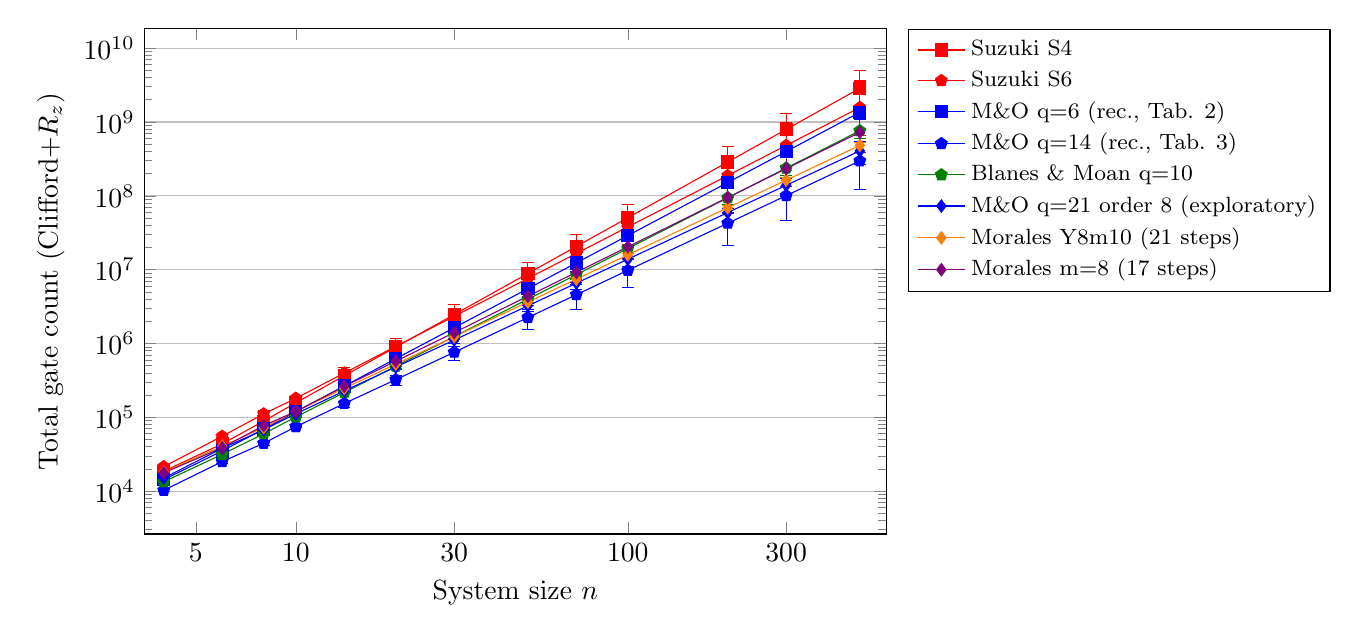
\begin{tikzpicture}
  \begin{loglogaxis}[
    width=11cm, height=8cm,
    xlabel={System size $n$},
    ylabel={Total gate count (Clifford+$R_z$)},
    xtick={5,10,30,100,300}, xticklabels={5,10,30,100,300},
    xmin=3.5, xmax=600,
    ymajorgrids=true,
    legend pos=outer north east,
    legend cell align=left,
    legend style={font=\footnotesize},
  ]
    % suzuki4: measured n, mean over seeds, bars min..max over seeds
    \addplot[red, solid, mark=square*, mark size=2.2pt, mark options={solid, fill=red}, error bars/.cd, y dir=both, y explicit, error bar style={solid}] coordinates {
      (4,18593.4) += (0,512.6) -= (0,419.4)
      (6,43617.6) += (0,419.4) -= (0,279.6)
      (8,88540) += (0,932) -= (0,932)
      (10,157275) += (0,3495) -= (0,1165)
    };
    \addlegendentry{Suzuki S4}
    % suzuki4: extrapolated, r = ceil(4.16533 n^1.50837), per step = 233/2 n + 0; bars min..max of per-seed fits
    \addplot[red, solid, mark=square*, mark size=2.2pt, mark options={solid, fill=red}, forget plot, error bars/.cd, y dir=both, y explicit, error bar style={solid}] coordinates {
      (10,157275)
      (14,365344) += (0,13048) -= (0,8155)
      (20,892390) += (0,48930) -= (0,27960)
      (30,2.46398e+06) += (0,199215) -= (0,108345)
      (50,8.86565e+06) += (0,984425) -= (0,524250)
      (70,2.06158e+07) += (0,2.71562e+06) -= (0,1.43528e+06)
      (100,5.04328e+07) += (0,7.74725e+06) -= (0,4.06585e+06)
      (200,2.86963e+08) += (0,5.66889e+07) -= (0,2.91716e+07)
      (300,7.93435e+08) += (0,1.77826e+08) -= (0,9.0171e+07)
      (500,2.85751e+09) += (0,7.38319e+08) -= (0,3.67499e+08)
    };
    % suzuki6: measured n, mean over seeds, bars min..max over seeds
    \addplot[red, solid, mark=pentagon*, mark size=2.2pt, mark options={solid, fill=red}, error bars/.cd, y dir=both, y explicit, error bar style={solid}] coordinates {
      (4,21460) += (0,0) -= (0,0)
      (6,55366.8) += (0,2575.2) -= (0,3862.8)
      (8,111163) += (0,13305.2) -= (0,12446.8)
      (10,180264) += (0,12876) -= (0,8584)
    };
    \addlegendentry{Suzuki S6}
    % suzuki6: extrapolated, r = ceil(1.64221 n^1.31614), per step = 1073/2 n + 0; bars min..max of per-seed fits
    \addplot[red, solid, mark=pentagon*, mark size=2.2pt, mark options={solid, fill=red}, forget plot, error bars/.cd, y dir=both, y explicit, error bar style={solid}] coordinates {
      (10,180264)
      (14,398083) += (0,75110) -= (0,52577)
      (20,912050) += (0,268250) -= (0,182410)
      (30,2.33378e+06) += (0,1.04618e+06) -= (0,627705)
      (50,7.59148e+06) += (0,5.06992e+06) -= (0,2.5752e+06)
      (70,1.65618e+07) += (0,1.37451e+07) -= (0,6.3468e+06)
      (100,3.78232e+07) += (0,3.85207e+07) -= (0,1.61486e+07)
      (200,1.88204e+08) += (0,2.7222e+08) -= (0,9.45313e+07)
      (300,4.8124e+08) += (0,8.35813e+08) -= (0,2.60578e+08)
      (500,1.57114e+09) += (0,3.37941e+09) -= (0,9.21707e+08)
    };
    % mo-q6: measured n, mean over seeds, bars min..max over seeds
    \addplot[blue, solid, mark=square*, mark size=2.2pt, mark options={solid, fill=blue}, error bars/.cd, y dir=both, y explicit, error bar style={solid}] coordinates {
      (4,14300) += (0,0) -= (0,0)
      (6,35062.5) += (0,412.5) -= (0,412.5)
      (8,69190) += (0,110) -= (0,990)
      (10,118800) += (0,825) -= (0,1925)
    };
    \addlegendentry{M\&O q=6 (rec., Tab. 2)}
    % mo-q6: extrapolated, r = ceil(3.52884 n^1.38766), per step = 275/2 n + 0; bars min..max of per-seed fits
    \addplot[blue, solid, mark=square*, mark size=2.2pt, mark options={solid, fill=blue}, forget plot, error bars/.cd, y dir=both, y explicit, error bar style={solid}] coordinates {
      (10,118800)
      (14,265650) += (0,5775) -= (0,7700)
      (20,621500) += (0,22000) -= (0,30250)
      (30,1.6335e+06) += (0,82500) -= (0,115500)
      (50,5.5275e+06) += (0,391875) -= (0,529375)
      (70,1.23489e+07) += (0,1.02988e+06) -= (0,1.386e+06)
      (100,2.893e+07) += (0,2.8325e+06) -= (0,3.74e+06)
      (200,1.51388e+08) += (0,1.9195e+07) -= (0,2.442e+07)
      (300,3.98558e+08) += (0,5.73375e+07) -= (0,7.14862e+07)
      (500,1.34949e+09) += (0,2.2385e+08) -= (0,2.72181e+08)
    };
    % mo-q14: measured n, mean over seeds, bars min..max over seeds
    \addplot[blue, solid, mark=pentagon*, mark size=2.2pt, mark options={solid, fill=blue}, error bars/.cd, y dir=both, y explicit, error bar style={solid}] coordinates {
      (4,10264.8) += (0,733.2) -= (0,488.8)
      (6,25112.1) += (0,2382.9) -= (0,1283.1)
      (8,44480.8) += (0,4399.2) -= (0,2932.8)
      (10,74542) += (0,1833) -= (0,1222)
    };
    \addlegendentry{M\&O q=14 (rec., Tab. 3)}
    % mo-q14: extrapolated, r = ceil(1.80948 n^1.12318), per step = 611/2 n + 0; bars min..max of per-seed fits
    \addplot[blue, solid, mark=pentagon*, mark size=2.2pt, mark options={solid, fill=blue}, forget plot, error bars/.cd, y dir=both, y explicit, error bar style={solid}] coordinates {
      (10,74542)
      (14,153972) += (0,8554) -= (0,17108)
      (20,323830) += (0,42770) -= (0,54990)
      (30,760695) += (0,155805) -= (0,174135)
      (50,2.24542e+06) += (0,672100) -= (0,702650)
      (70,4.57639e+06) += (0,1.7108e+06) -= (0,1.66803e+06)
      (100,9.776e+06) += (0,4.3381e+06) -= (0,4.0326e+06)
      (200,4.25256e+07) += (0,2.5662e+07) -= (0,2.10184e+07)
      (300,1.00448e+08) += (0,7.08454e+07) -= (0,5.37986e+07)
      (500,2.97252e+08) += (0,2.49746e+08) -= (0,1.7383e+08)
    };
    % bm-q10: measured n, mean over seeds, bars min..max over seeds
    \addplot[green!50!black, solid, mark=pentagon*, mark size=2.2pt, mark options={solid, fill=green!50!black}, error bars/.cd, y dir=both, y explicit, error bar style={solid}] coordinates {
      (4,13378.6) += (0,797.4) -= (0,88.6)
      (6,31497.3) += (0,398.7) -= (0,930.3)
      (8,59893.6) += (0,354.4) -= (0,1417.6)
      (10,101226) += (0,2879.5) -= (0,1550.5)
    };
    \addlegendentry{Blanes \& Moan q=10}
    % bm-q10: extrapolated, r = ceil(2.3688 n^1.28299), per step = 443/2 n + 0; bars min..max of per-seed fits
    \addplot[green!50!black, solid, mark=pentagon*, mark size=2.2pt, mark options={solid, fill=green!50!black}, forget plot, error bars/.cd, y dir=both, y explicit, error bar style={solid}] coordinates {
      (10,101226)
      (14,217070) += (0,15505) -= (0,6202)
      (20,491730) += (0,57590) -= (0,31010)
      (30,1.24262e+06) += (0,205995) -= (0,106320)
      (50,3.97592e+06) += (0,941375) -= (0,443000)
      (70,8.55876e+06) += (0,2.44979e+06) -= (0,1.08535e+06)
      (100,1.93148e+07) += (0,6.5564e+06) -= (0,2.7909e+06)
      (200,9.40046e+07) += (0,4.22622e+07) -= (0,1.6834e+07)
      (300,2.37226e+08) += (0,1.22932e+08) -= (0,4.70466e+07)
      (500,7.61406e+08) += (0,4.63821e+08) -= (0,1.69004e+08)
    };
    % mo-o8-q21: measured n, mean over seeds, bars min..max over seeds
    \addplot[blue, solid, mark=diamond*, mark size=2.2pt, mark options={solid, fill=blue}, error bars/.cd, y dir=both, y explicit, error bar style={solid}] coordinates {
      (4,15023) += (0,1267) -= (0,543)
      (6,38010) += (0,2715) -= (0,2715)
      (8,67694) += (0,4706) -= (0,2534)
      (10,111315) += (0,6335) -= (0,2715)
    };
    \addlegendentry{M\&O q=21 order 8 (exploratory)}
    % mo-o8-q21: extrapolated, r = ceil(1.93865 n^1.0989), per step = 905/2 n + 0; bars min..max of per-seed fits
    \addplot[blue, solid, mark=diamond*, mark size=2.2pt, mark options={solid, fill=blue}, forget plot, error bars/.cd, y dir=both, y explicit, error bar style={solid}] coordinates {
      (10,111315)
      (14,228060) += (0,19005) -= (0,12670)
      (20,479650) += (0,63350) -= (0,36200)
      (30,1.11315e+06) += (0,244350) -= (0,122175)
      (50,3.23538e+06) += (0,1.086e+06) -= (0,497750)
      (70,6.55672e+06) += (0,2.75572e+06) -= (0,1.20365e+06)
      (100,1.38465e+07) += (0,7.059e+06) -= (0,2.94125e+06)
      (200,5.92775e+07) += (0,4.17205e+07) -= (0,1.5928e+07)
      (300,1.38872e+08) += (0,1.14844e+08) -= (0,4.16752e+07)
      (500,4.05666e+08) += (0,4.04535e+08) -= (0,1.37108e+08)
    };
    % morales-y8m10: measured n, mean over seeds, bars min..max over seeds
    \addplot[orange, solid, mark=diamond*, mark size=2.2pt, mark options={solid, fill=orange}, error bars/.cd, y dir=both, y explicit, error bar style={solid}] coordinates {
      (4,18100) += (0,0) -= (0,0)
      (6,40725) += (0,0) -= (0,0)
      (8,72400) += (0,0) -= (0,0)
      (10,120818) += (0,1357.5) -= (0,3167.5)
    };
    \addlegendentry{Morales Y8m10 (21 steps)}
    % morales-y8m10: extrapolated, r = ceil(1.98514 n^1.12271), per step = 905/2 n + 0; bars min..max of per-seed fits
    \addplot[orange, solid, mark=diamond*, mark size=2.2pt, mark options={solid, fill=orange}, forget plot, error bars/.cd, y dir=both, y explicit, error bar style={solid}] coordinates {
      (10,120818)
      (14,247065) += (0,6335) -= (0,6335)
      (20,524900) += (0,9050) -= (0,27150)
      (30,1.23532e+06) += (0,40725) -= (0,95025)
      (50,3.64262e+06) += (0,158375) -= (0,339375)
      (70,7.44362e+06) += (0,348425) -= (0,823550)
      (100,1.58375e+07) += (0,905000) -= (0,1.991e+06)
      (200,6.88705e+07) += (0,5.068e+06) -= (0,1.0679e+07)
      (300,1.629e+08) += (0,1.34392e+07) -= (0,2.81002e+07)
      (500,4.8146e+08) += (0,4.57025e+07) -= (0,9.29888e+07)
    };
    % morales-m8: measured n, mean over seeds, bars min..max over seeds
    \addplot[violet, solid, mark=diamond*, mark size=2.2pt, mark options={solid, fill=violet}, error bars/.cd, y dir=both, y explicit, error bar style={solid}] coordinates {
      (4,17688) += (0,0) -= (0,0)
      (6,38692.5) += (0,1105.5) -= (0,1105.5)
      (8,77237.6) += (0,2358.4) -= (0,3537.6)
      (10,119762) += (0,5527.5) -= (0,5527.5)
    };
    \addlegendentry{Morales m=8 (17 steps)}
    % morales-m8: extrapolated, r = ceil(1.995 n^1.22085), per step = 737/2 n + 0; bars min..max of per-seed fits
    \addplot[violet, solid, mark=diamond*, mark size=2.2pt, mark options={solid, fill=violet}, forget plot, error bars/.cd, y dir=both, y explicit, error bar style={solid}] coordinates {
      (10,119762)
      (14,263109) += (0,20636) -= (0,25795)
      (20,574860) += (0,81070) -= (0,81070)
      (30,1.40398e+06) += (0,298485) -= (0,254265)
      (50,4.36672e+06) += (0,1.3266e+06) -= (0,1.06865e+06)
      (70,9.20882e+06) += (0,3.40494e+06) -= (0,2.5795e+06)
      (100,2.03412e+07) += (0,8.9177e+06) -= (0,6.44875e+06)
      (200,9.47782e+07) += (0,5.56435e+07) -= (0,3.63341e+07)
      (300,2.3326e+08) += (0,1.5886e+08) -= (0,9.77262e+07)
      (500,7.25208e+08) += (0,5.85546e+08) -= (0,3.34414e+08)
    };
  \end{loglogaxis}
\end{tikzpicture}
